\section{Internet of Things}

\paragraph{Safety vs. Security}
Safety is the protection against random, unwanted incidents - resulting from coincidences or driven by the environment (which does not adapt to bypass safety measures). Security is the protection against intended incidents - resulting from a deliberate planned act and driven by targeted attacker.

%TODO: intro slides? examples, generally how important?

\begin{figure}[h]
	\centering
	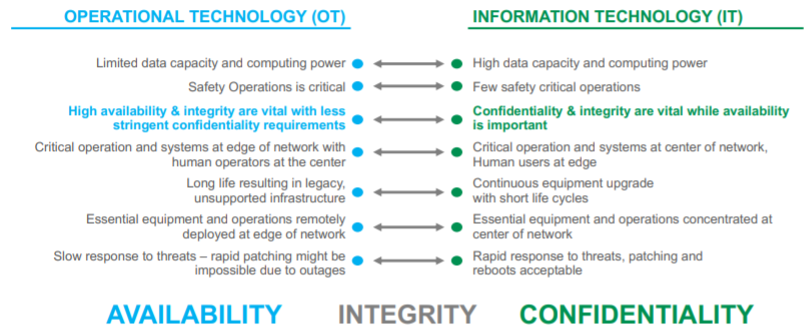
\includegraphics[scale=0.8]{images/913-otvsit.PNG}
	\caption{Key differences between operational and information technology.}
	\label{fig:ot}
\end{figure}

\paragraph{Attack Surface}
IoT connects innumerable everyday devices and systems. Devices can have insecure software / vulnerabilities and insecure defaults, cheap components, be lacking of an update mechanism. Furthermore, since they're replicated, finding a fault in one can give access to all (no unique identity). Backend service is the central control and can be attacked in regards to data (breaches, privacy, etc.). Both ends are connected with by an insecure communication channel (weak or no crypto, lack of authentication, etc.). Now, closed systems are opened up to remote access and control!

IoT devices are perceived to have very low risk in comparison to a computer. An attacker can exploit this risk perception (easy targets).

IoT devices are mainly designed to have high availability with safety but no security. They need continued security maintenance. Also, certification timeline is often outpaced by cyber security (patches make a certification unusable).

\begin{figure}[h]
	\centering
	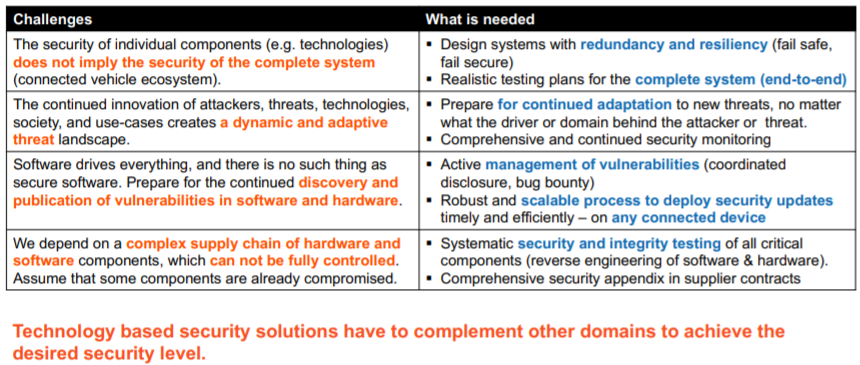
\includegraphics[scale=0.8]{images/913-conclusion.PNG}
	\caption{Summary of IoT lecture.}
	\label{fig:conclusion}
\end{figure}